\chapter{Preliminaries and Introduction\label{sec:introduction}}
\section{Overview}
The Project title states "Real time Video based Pakistan Sign Language Recognition". Real time gives the sense that system will be producing output just as it is given an input i.e. very small time laps. Real time performance is one of the most demanded quality of a machine learning based software product. The video based approach means that we will be using multiple videos of signs for training (tuning) the model in order to use this model for purpose of prediction of an unseen example (practiced sign). The segment "Pakistan Sign Language" conveys that the signs that will be predicted by the system are of Pakistan Sign Language.  \\
The signer will be doing the sign in front of a Kinect Camera device. This is passed to the system. System evaluates the sign on model already built and outputs the text against the sign. Many such systems are developed and many more are in form of complete commercial products e.g. Motion Savvy and Microsoft Kinect Sign Language Recognition. This product does not intend to challenge the previous work rather this is an attempt to expand the cloud of this technology to Pakistan Sign Language Recognition.


\section{Motivation}
Around 360 million people around the world (5\% of world’s population) are suffering from some kind of hearing loss and many are those who cannot speak. This creates a sub-conscious barrier between such disabled persons and rest of the society. Such subjects use Sign languages to communicate. Many countries have developed technologies that could help such participants remove this barrier in order to get a healthy and transparent society. But sadly there’s been very little work done in Pakistan Sign Language (PSL) technologies. PSL Recognition systems created till now are limited to numbers and other signs like directions, colors and body parts etc. Most of PSL technologies are static sign language recognition. \\
System proposed is a dynamic sign language recognition technology that takes live video of PSL signs and predicts its meanings in textual form. This can contribute in flourishing of PSL and disabled people. 


\section{ Objective}
The objective of this project is to come up with a technology that takes visual input (live video) of a sign being practiced in Pakistan Sign Language and predicts what it means in textual form.


\section{ Target Group}
The intended subjects of this technology are the people who suffer from any kind of hearing loss and knows Pakistan Sign Language and those who want to communicate to a mute person and do not know Pakistan Sign Language.

\section{ Problem Statement}
Hearing impaired or mute people are cornered due to inability of communication with other people. Currently in Pakistan, there is no technology that could help them with communication. There is work done on this technology but that is only limited to static sign inputs. There is needed a system that works on dynamic inputs and could serve the purpose of Sign to text translation in real time.

\section{Solution proposed}
A video based machine learning approach is proposed that takes in video in real time and predicts the text against a sign practiced in video. This system can be trained on some pre-specified set of signs and a model for classification is established. Later a sign video can be evaluated on this model and classified accordingly.
\subsection{Motivation to use Kinect device for SLR}
The conjunction of depth map and color image from Kinect sensor could produce great contribution for sign language recognition in three aspects. First, with the depth map, back-ground modeling becomes more simple and robust. We can easily and accurately extract human body part from color images. Second, in previous 2-D solutions, how to track hands is a difficult task. However, the skeleton information, developed from depth map, can be utilized to locate the positions of hands robustly and in real time. Third, beyond the traditional 2-D features, Kinect senor can provide some novel 3-D features, which are quite useful and hence and improve the performance of sign language recognition. These advantages will emerge in our following experimental results.
\subsection{Motivation to use features from hand finger and skeleton}
These actually gives a visualization of how a hand performs a sign in physical and how an interpreter can interpret it. As a finger is bent, its distance from the successive finger changes, angle of the defect (joint) is also effected and the distance between the joint and a hull around the hand also changes. So a single moves provides uniqueness in all three dimensions of main features. This justifies that these features would be good to be used for unique pattern identification. 


\begin{figure}[!htb]
	\begin{center}
		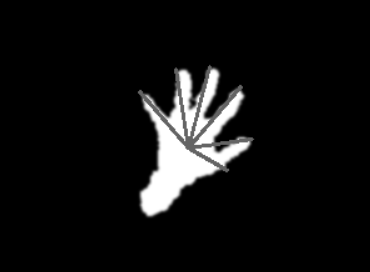
\includegraphics{ThesisFigs/skeletnon}
		\caption{Skeletnon of Hand }\label{fig:Skeletnon of Hand}
	\end{center}
\end{figure}


\subsection{Motivation to use Random Forest Classifier}
Random forest is actually an ensemble based learning in which we used multiple classifiers each a decision tree, and then predict the sign using all those trees. In the end, we assign probabilities to each class as with the ratio of predicted by trees and lastly we pick it based on the probability.
Moreover, our data is non-categorical or numeric (ordinal). Random works really well when the features are known. For each of the tree, it would apply multiple splits based on minimum entropy and maximum information gain.
Do in this case, Prediction is simpler i.e. just parse through the tree and predict the leaf class. Prediction does not take too much time. Prediction is ensemble so not a much chances to over fit on some class.

\section{Scope:}
This project can be installed to different scope domains like in hospital for training, communication and prescriptions. Following scenarios can use a furnished and modified form of this project.
\begin{itemize}
\item[•]\textbf{	Training:}\newline
There are patients in the hospital who have partial disability to speak, they use a bit of sign language to communicate. Such people can use the product. Also there are others who are deaf but they need to be trained how to speak i.e. how to twist the tongue, clump the lips and direct your voice. So they can be trained and communicated using this sign language machine by an ordinary person who does not know sign language. Moreover there are others who are complete deaf or mute, they also use sign language. For each of the above case, different sets of sentences could be selected for communication and make a custom model and use it.


	

\item[•]\textbf{	Communication with doctor:}\newline 
A doctor who does not know sign language can be made able to understand the problems of the mute patient. We can also enable the doctor to do the prescription to a deaf person using this machine by adding feature to replace the words with sign itself.
\end{itemize}
\section{Some related famous products: }
Following are the examples of already available state of the art products that are available to general public. Their technology in some aspects to the technology of the concerned project.
\begin{itemize}
	\item DICTA sign  \cite{DICTAsign}
	\item Motion Savvy  \cite{MotionSavvy}
	\item MS Sign Language Translator \cite{MSSignLanguageTranslator}
\end{itemize}


\section{	SWOT Analysis }

\begin{center}
	\begin{tabular}{ |p{7cm}|p{7cm}| } 
		\hline
		\textbf{Strengths} & \textbf{Weaknesses}\\
		\hline
		\textbf{Performance :} 
		Now a days, performance is main concern. System under consideration performs well in a constrained environment as specified in weaknesses. \newline 
		\textbf{Time:} \newline 
		This system works in real time so no more time lapses.\newline 
		\textbf{Reliability:} \newline
		Reliability is the best a promise a product can make to its users. The system assures reliability by assuring all software development measures and steps. \newline
		\textbf{Luminance: }\newline 
		Almost all other systems serving the purpose are confined by luminance i.e. proper lightning is necessary for system to work properly. Which is not the case with the system being proposed.
		& \textbf{Supplements:} \newline
		A Kinect Camera device is needed in order to get input as no ordinary camera can serve the purpose of depth frame capturing.  \newline
		\textbf{Portability:}\newline
		A laptop is enough to get the system working but it needs a Kinect Camera to be available also. Which is not an every place utility so needed to be carried along. More else the system is going to need to be configured before use. Not an instant plug and play module.\newline
		\textbf{Distance:} \newline
		The system works only when the sign is being practiced at a constrained distance of \# ft. Else way, the sign goes undetected and hence can’t be processed. \\
	
		\hline
		\textbf{Opportunities} &  \textbf{ Threats:}\\
		
		 \hline 
		 open source software is easily available to edit and extend. Their debugging is also easy, as it is open source so many people can extend it for their purposes and can debug. &
		  System pose no physical or social threats to anybody. It will only benefit those who use it. But yes, in a way, this may prevent someone to learn PSL by themselves  \\
		\hline
	\end{tabular}
\end{center}



